\documentclass[tikz,12pt,border=2pt]{standalone}
\usepackage[T1]{fontenc}
\usepackage[scaled=0.92]{helvet}
\renewcommand{\familydefault}{\sfdefault}
\usetikzlibrary{arrows.meta,positioning,calc}
\definecolor{accent}{RGB}{31,84,140}
\definecolor{accentlight}{RGB}{200,214,232}
\begin{document}
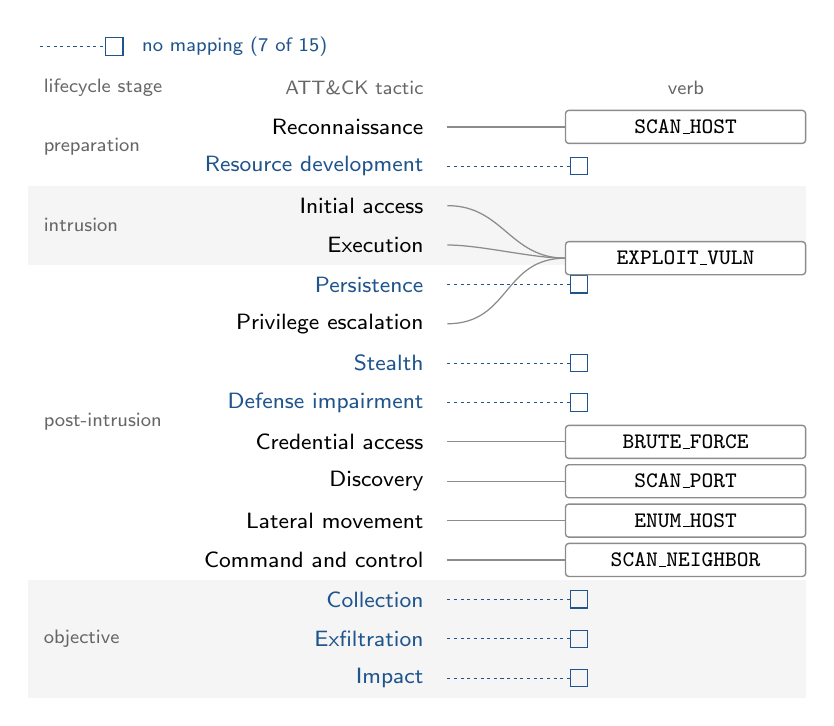
\begin{tikzpicture}[x=1cm,y=1cm,>={Stealth[length=1.6mm]},every node/.style={font=\footnotesize}]
\node[anchor=west,font=\scriptsize,text=black!60] at (0.08,-0.250) {preparation};
\fill[black!4] (0.00,-0.75) rectangle (9.88,-1.75);
\node[anchor=west,font=\scriptsize,text=black!60] at (0.08,-1.250) {intrusion};
\node[anchor=west,font=\scriptsize,text=black!60] at (0.08,-3.750) {post-intrusion};
\fill[black!4] (0.00,-5.75) rectangle (9.88,-7.25);
\node[anchor=west,font=\scriptsize,text=black!60] at (0.08,-6.500) {objective};
\draw[accent,line width=0.4pt,dash pattern=on 1.1pt off 1.3pt] (0.16,1.020) -- (0.99,1.020);
\draw[accent,line width=0.4pt] (0.99,0.910) rectangle (1.21,1.130);
\node[anchor=west,font=\scriptsize,text=accent] at (1.33,1.020) {no mapping (7 of 15)};
\node[anchor=west,font=\scriptsize,text=black!60] at (0.08,0.50) {lifecycle stage};
\node[anchor=east,font=\scriptsize,text=black!60] at (5.15,0.50) {ATT\&CK tactic};
\node[anchor=center,font=\scriptsize,text=black!60] at (8.36,0.50) {verb};
\node[anchor=east,text=black] at (5.15,0.000) {Reconnaissance};
\node[anchor=east,text=accent] at (5.15,-0.500) {Resource development};
\node[anchor=east,text=black] at (5.15,-1.000) {Initial access};
\node[anchor=east,text=black] at (5.15,-1.500) {Execution};
\node[anchor=east,text=accent] at (5.15,-2.000) {Persistence};
\node[anchor=east,text=black] at (5.15,-2.500) {Privilege escalation};
\node[anchor=east,text=accent] at (5.15,-3.000) {Stealth};
\node[anchor=east,text=accent] at (5.15,-3.500) {Defense impairment};
\node[anchor=east,text=black] at (5.15,-4.000) {Credential access};
\node[anchor=east,text=black] at (5.15,-4.500) {Discovery};
\node[anchor=east,text=black] at (5.15,-5.000) {Lateral movement};
\node[anchor=east,text=black] at (5.15,-5.500) {Command and control};
\node[anchor=east,text=accent] at (5.15,-6.000) {Collection};
\node[anchor=east,text=accent] at (5.15,-6.500) {Exfiltration};
\node[anchor=east,text=accent] at (5.15,-7.000) {Impact};
\draw[black!45,line width=0.45pt] (5.33,0.000) .. controls +(0.34,0) and +(-0.34,0) .. (6.83,0.000);
\draw[accent,line width=0.4pt,dash pattern=on 1.1pt off 1.3pt] (5.33,-0.500) -- (6.89,-0.500);
\draw[accent,line width=0.4pt] (6.89,-0.610) rectangle (7.11,-0.390);
\draw[black!45,line width=0.45pt] (5.33,-1.000) .. controls +(0.71,0) and +(-0.71,0) .. (6.83,-1.667);
\draw[black!45,line width=0.45pt] (5.33,-1.500) .. controls +(0.43,0) and +(-0.43,0) .. (6.83,-1.667);
\draw[accent,line width=0.4pt,dash pattern=on 1.1pt off 1.3pt] (5.33,-2.000) -- (6.89,-2.000);
\draw[accent,line width=0.4pt] (6.89,-2.110) rectangle (7.11,-1.890);
\draw[black!45,line width=0.45pt] (5.33,-2.500) .. controls +(0.80,0) and +(-0.80,0) .. (6.83,-1.667);
\draw[accent,line width=0.4pt,dash pattern=on 1.1pt off 1.3pt] (5.33,-3.000) -- (6.89,-3.000);
\draw[accent,line width=0.4pt] (6.89,-3.110) rectangle (7.11,-2.890);
\draw[accent,line width=0.4pt,dash pattern=on 1.1pt off 1.3pt] (5.33,-3.500) -- (6.89,-3.500);
\draw[accent,line width=0.4pt] (6.89,-3.610) rectangle (7.11,-3.390);
\draw[black!45,line width=0.45pt] (5.33,-4.000) .. controls +(0.34,0) and +(-0.34,0) .. (6.83,-4.000);
\draw[black!45,line width=0.45pt] (5.33,-4.500) .. controls +(0.34,0) and +(-0.34,0) .. (6.83,-4.500);
\draw[black!45,line width=0.45pt] (5.33,-5.000) .. controls +(0.34,0) and +(-0.34,0) .. (6.83,-5.000);
\draw[black!45,line width=0.45pt] (5.33,-5.500) .. controls +(0.34,0) and +(-0.34,0) .. (6.83,-5.500);
\draw[accent,line width=0.4pt,dash pattern=on 1.1pt off 1.3pt] (5.33,-6.000) -- (6.89,-6.000);
\draw[accent,line width=0.4pt] (6.89,-6.110) rectangle (7.11,-5.890);
\draw[accent,line width=0.4pt,dash pattern=on 1.1pt off 1.3pt] (5.33,-6.500) -- (6.89,-6.500);
\draw[accent,line width=0.4pt] (6.89,-6.610) rectangle (7.11,-6.390);
\draw[accent,line width=0.4pt,dash pattern=on 1.1pt off 1.3pt] (5.33,-7.000) -- (6.89,-7.000);
\draw[accent,line width=0.4pt] (6.89,-7.110) rectangle (7.11,-6.890);
\draw[black!45,line width=0.5pt,fill=white,rounded corners=1.2pt] (6.83,-0.210) rectangle (9.88,0.210);
\node[anchor=center] at (8.355,0.000) {\texttt{SCAN\_HOST}};
\draw[black!45,line width=0.5pt,fill=white,rounded corners=1.2pt] (6.83,-1.877) rectangle (9.88,-1.457);
\node[anchor=center] at (8.355,-1.667) {\texttt{EXPLOIT\_VULN}};
\draw[black!45,line width=0.5pt,fill=white,rounded corners=1.2pt] (6.83,-4.210) rectangle (9.88,-3.790);
\node[anchor=center] at (8.355,-4.000) {\texttt{BRUTE\_FORCE}};
\draw[black!45,line width=0.5pt,fill=white,rounded corners=1.2pt] (6.83,-4.710) rectangle (9.88,-4.290);
\node[anchor=center] at (8.355,-4.500) {\texttt{SCAN\_PORT}};
\draw[black!45,line width=0.5pt,fill=white,rounded corners=1.2pt] (6.83,-5.210) rectangle (9.88,-4.790);
\node[anchor=center] at (8.355,-5.000) {\texttt{ENUM\_HOST}};
\draw[black!45,line width=0.5pt,fill=white,rounded corners=1.2pt] (6.83,-5.710) rectangle (9.88,-5.290);
\node[anchor=center] at (8.355,-5.500) {\texttt{SCAN\_NEIGHBOR}};
\end{tikzpicture}
\end{document}
